\documentclass{book}
\usepackage[latin1]{inputenc}    
\usepackage[T1]{fontenc}
\usepackage[german]{babel}     
\usepackage{graphicx}
\pagestyle{headings}
\usepackage[top=2cm, bottom=3cm, left=2cm, right=2cm]{geometry}
\usepackage{wrapfig}
\usepackage{hyperref}

\hypersetup{
backref=true, %permet d'ajouter des liens dans...
pagebackref=true,%...les bibliographies
hyperindex=true, %ajoute des liens dans les index.
colorlinks=true, %colorise les liens
breaklinks=true, %permet le retour � la ligne dans les liens trop longs
urlcolor= black, %couleur des hyperliens
linkcolor= black, %couleur des liens internes
bookmarks=true, %cr�� des signets pour Acrobat
bookmarksopen=true, %si les signets Acrobat sont cr��s,
%les afficher compl�tement.
pdftitle={Designing eines Computerspiels}, %informations apparaissant dans
pdfauthor={Samuel Gauthier}, %dans les informations du document
pdfsubject={Windows XP} %sous Acrobat.
}

\begin{document}
\begin{titlepage}
\centering

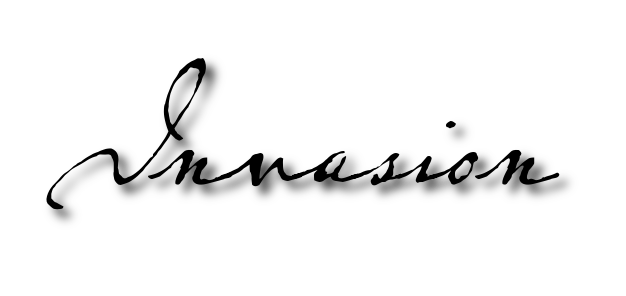
\includegraphics[width=.75\textwidth]{logo.png}

\Huge{Designing eines Computerspiels\\ \vspace{300pt}}
\Large{Samuel Gauthier\\Maturarbeit 2012\\}
\small{\textit{Betreuer:} Thomas Vogelsanger\\}
\end{titlepage}
\tableofcontents
\frontmatter
\chapter{Vorwort}
Als ich 4 war bekam ich meinen ersten eigenen Computer: ein Maxdata 286 mit 12Mhz Prozessor 20MB Festplatte 1MB Ram. Auf dessen lief noch DOS. Von dieser Zeit an, begann ich die IT Welt zu entdecken. Mein erstes Spiele war das Golf Spiel PGA Tour 96. Ich verbrachte Stunden um zu verstehen wie man am besten Golf spielen konnte. Ein anderes Spiel war ein Spiel das zu zweit gespielt wurde und indem das Ziel den gegnerischen Affen mit Bananen zu beschiessen war; Wind und Gravitation kamen auch in Frage. Als ich manchmal genug von spielen hatte probierte ich alle m�glichen Einstellungen des Computers aus. Nat�rlich von Zeit st�rzte meinen Computer ab und mein Vater musste ihn wieder herrichten. Einige Jahre sp�ter bekam ich meinen zweiten Computer: ein --- mit mit ---Mhz Prozessor ---MB Festplatte ---MB Ram. (Schon hier sieht man die rasante Entwicklung der Informatik die in den n�chsten Jahren noch gr�sser geworden ist.) Danach spielte ich mit dem Valdo spiel. Ein "Adventure Thinking" Game. Auch hier brachte ich viele Zeit damit. Z.B. als der Lothard Sturm die ganze Schweiz durchsch�ttelte spielten meinen Bruder, meinen Vater und ich mit diesem Spiel. Doch weil es von Zeit zu Zeit Stromst�rungen gab, machte der Computer Reboots. Und weil der Spielstand nicht gesichert wurde m�ssten wir immer neu anfangen und lernten so fast das ganze Spiel auswendig. Nach diesem Spiel kam eines meiner Liebsten Spiele und das meine Maturarbeit sehr beeinflusst hat: Age of Empires 2. Erstaunlicherweise lernte ich mit diesem Spiel die ber�hmtesten Geschichten der damaligen gr�ssten M�chten zu kennen. Die Entwickler hatten n�mlich mehrere reale historische Kampagnen geschaffen wie z.B. "Die Jungfrau von Orleans" (eine Kampagne der Befreiung Frankreichs von den Engl�ndern im 100Jahren Krieg) oder "Genghis Kahn". In den n�chsten Jahren  
\newline
\newline
Ich m�chte mich hier bei den folgenden Personen ganz herzlich bedanken: Julien Burkhard, ohne ihn w�re hier kein Spiel entstanden, Herr Voglesanganger f�r seine Betreuung, meine Freude die das Spiel getestet haben und nat�rlich auch meine Familie die mir konstante Unterst�tzung gab und immer nachfragte wo ich mit meiner Maturarbeit sei.
 
\mainmatter
\chapter{Einf�hrung}
\chapter{Das Spiel}
\chapter{Blender}
\chapter{Textures}
\chapter{Website}

\backmatter
\chapter{Nachwort}
\chapter{Quellen}

\end{document}